\documentclass[a4paper,norsk]{article}
\usepackage{preamble}

\begin{document}

\subsection{Om An og Faltinsens artikkel: \emph{Linear free-surface effects on a horisontally submerged and perforated 2D thin plate in finite and infinite water depths}}

An $\&$ Faltinsen \cite{faltinsen} ser på en horisontal, uendelig tynn plate i 2D,
nedsunket i et fluid av både endelig og uendelig dybde. Oppsettet er illustrert
i figur (\ref{fig::faltinsen}). I denne artikkelen studerer de diffraksjon av
bølger i tillegg til tvugne oscillasjoner i hiv og rull. Disse oscillasjonene
gir opphav til addert masse- og dempningseffekter.

Strømningen på grunn av platen blir her representert av en virveldistribusjon 
langs $y=b$, $-L/2 \leq x \leq L/2$. Platens tilstedeværelse representeres av en
Green-funksjon lagt fram av Wehausen $\&$ Laitone \cite{wehausen}, som
tilfredsstiller betingelsene ved lineær fri overflate, 
\begin{align}
  \pder{\phi}{y} - \nu\phi = 0 \hspace{3mm} \text{on} \hspace{3mm} y = 0 \,,
           \hspace{3mm} \nu=\frac{\omega^2}{g}
\end{align}
uendelig dyp
\begin{align}
  \pder{\phi}{y} \rightarrow 0 \hspace{3mm} \text{when} \hspace{3mm}
                                         y \rightarrow -\infty
\end{align}
og radiasjon
\begin{align}
  \lim_{x\rightarrow\pm\infty} \left( \pder{}{x}\mp i\nu \right)
  \begin{pmatrix}
    \phi_r \\ \phi_d
  \end{pmatrix} = 0 \;.
\end{align}

An $\&$ Faltinsen tar høyde for porøsitet ved å anvende en kvadratisk trykkrelasjon
foreslått av Molin \cite{molin} på formen
\begin{align}
  \Delta p = \frac{1-\tau}{2\mu\tau^2}\rho|\vec{V}|\vec{V} \;.
\end{align}
Her er $\tau$ en porøsitetsparameter som tar verdier mellom 0 og 1, hvor $\tau=0$
betyr ingen gjennomstrømning, og ved $\tau=1$ er geometrien helt åpen. Videre er
$\mu$ en utslippskoeffisient som typisk har verdi mellom $0.5$ og $1.0$.
$\vec{V}$ .....?

\begin{figure}
\centering
\begin{subfigure}{.5\textwidth}
  \centering
  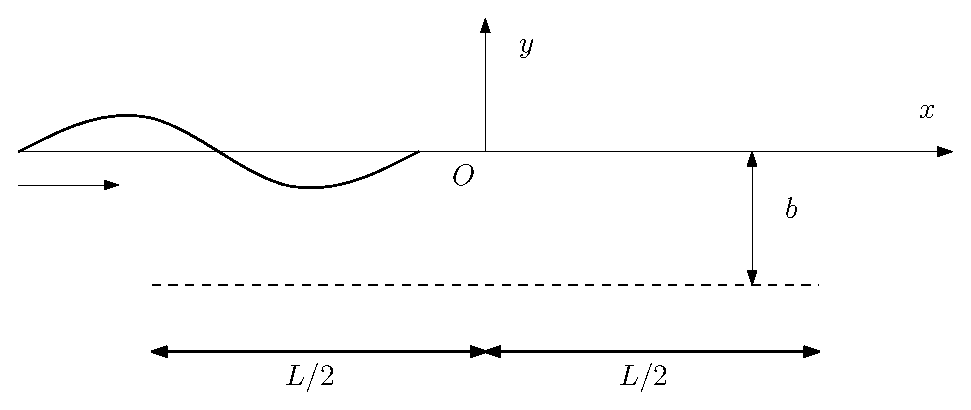
\includegraphics[width=0.95\linewidth]{horisontal_plate.eps}
  \caption{}
  \label{fig::faltinsen1}
\end{subfigure}%
\begin{subfigure}{.5\textwidth}
  \centering
  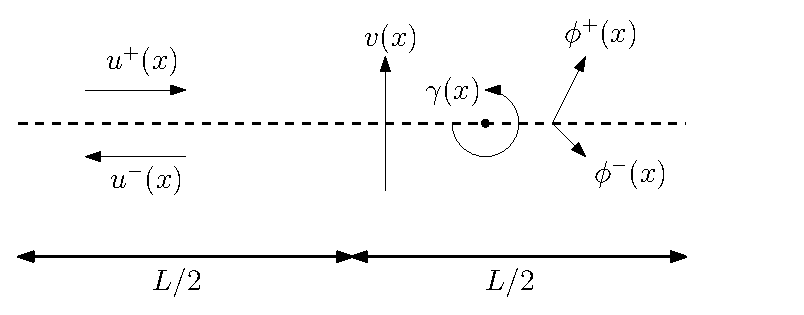
\includegraphics[width=0.95\linewidth]{horisontal_plate_closeup.eps}
  \caption{}
  \label{fig::faltinsen2}
\end{subfigure}
\caption{\textbf{Fig.} 1, s. 222 i \cite{faltinsen}. (a) Geometri og plassering av plate. (b) Kompleks amplitude av hastighetspotensialet $\phi$, horisontal hastighet $u^\pm$ og vertikal strømning $v$ gjennom perforeringen.}
\label{fig::faltinsen}
\end{figure}

\begin{thebibliography}{99} %

\bibitem{faltinsen}
  S. An, O. Faltinsen
  \emph{Linear free-surface effects on a horisontally submerged and perforated 2D thin plate in finite and infinite water depths},
  Applied Ocean Research,
  vol. 37 (2012),
  p. 220-234

\bibitem{molin}
  B. Molin,
  \emph{Hydrodynamic modeling of perforated structures},
  Applied Ocean Research,
  vol. 33 (2011),
  p. 1-11

\bibitem{wehausen}
  Wehausen JV and Laitone EV,
  \emph{Surface waves},
  online edition (1960)

\end{thebibliography}

\end{document}
